\newcommand{\aanleiding}{}

\begin{wrapfigure}{r}{4cm}
  \begin{center}
    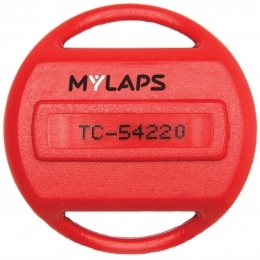
\includegraphics[width=4cm]{style/images/transponder}
  \end{center}
  \caption{MyLaps ProFlex transponder, op schaal}
  \label{fig:transponder}
  \vspace{15mm}
\end{wrapfigure}

In baansporten is de laatste jaren een ontwikkeling gaande om tijdregistratie te digitaliseren door het gebruik van transponders zoals de \mylaps ProFlex transponder in figuur~\ref{fig:transponder} en detectielussen die in de baan zijn verwerkt, wat te zien is in figuur~\ref{fig:detection-loop}. Door deze ontwikkeling zijn nieuwe mogelijkheden ontstaan om ook naast het wedstrijdmoment de sportprestaties in te zien. Het constateren van de hierna genoemde nieuwe mogelijkheden vormde de aanleiding voor dit project.

\begin{wrapfigure}{r}{4cm}
  \begin{center}
    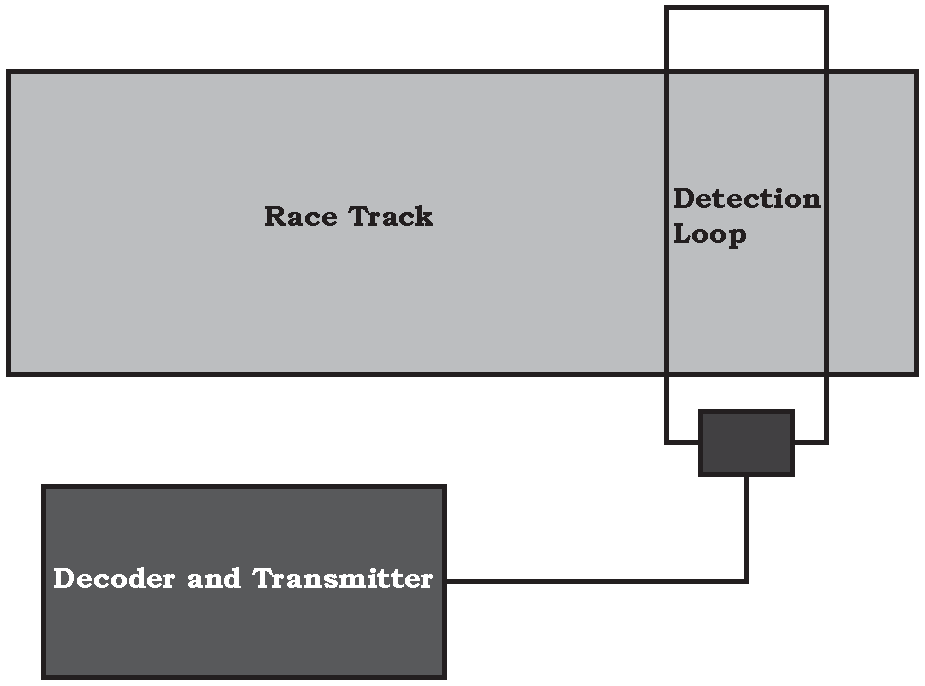
\includegraphics[width=4cm]{style/images/DetectionLoop}
  \end{center}
  \caption{Een schema van een detectielus en en decoder}
  \label{fig:detection-loop}
  \vspace{5mm}
\end{wrapfigure}

Een grote speler op de tijdregistratiemarkt is \mylaps\footnote{\url{http://www.mylaps.com}}. Dit bedrijf installeert en beheert detectielussen en is actief bij diverse sporten zoals schaatsen, wielrennen, zwemmen, atletiek en diverse motorsporten. Bij sporten met permanente banen liggen de detectielussen het gehele jaar in de baan. Er bestaat de mogelijkheid om op de website van \mylaps doorkomsttijden in te zien. De informatie die uit deze tijden is af te leiden, wordt door sporters die zich willen blijven verbeteren als erg waardevol gezien, waardoor er steeds meer getraind wordt met deze transponders.

\begin{figure}
  \begin{center}
    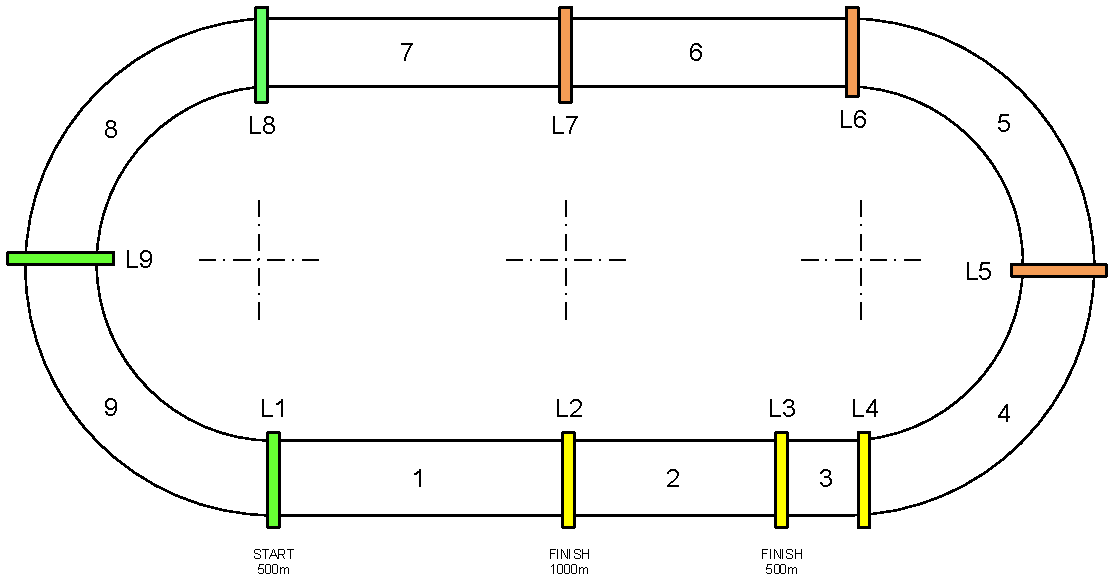
\includegraphics[width=0.8\textwidth]{style/images/BaanoverzichtHaarlem}
  \end{center}
  \caption{L1 tot en met L9 zijn de negen \mylaps detectielussen in Haarlem}
  \label{fig:track-transponders}
\end{figure}

Voor aanvang van het seizoen installeert \mylaps een aantal detectielussen in de baan. De lussen bevinden zich in het ijs of onder het houten oppervlak van een baanwielrenbaan. Elke lus heeft een elektromagnetisch veld. Wanneer een sporter met transponder over dat veld heen rijdt, wordt de transponder geactiveerd en stuurt deze een unieke puls, die vervolgens door de lus wordt opgevangen. De \mylaps X2 Server die aan de detectielussen zit aangesloten stuurt vervolgens het signaal door naar de \mylaps Cloud.

Het huidige gebruik van transponders - buiten wedstrijden - is voornamelijk achteraf, terwijl juist tijdens de training zowel sporter als coach het meeste bezig zijn met de prestaties. Het is daarom wenselijk om de resultaten in realtime door te geven aan coaches en sporters zelf.

Op veel banen zijn meerdere detectielussen geïnstalleerd, terwijl er op de website van \mylaps slechts één wordt ontsloten omdat \mylaps dit niet ziet als haar `core business'. In Thialf, de schaatsbaan in Heerenveen, Friesland, liggen bijvoorbeeld twaalf detectielussen, in Haarlem (figuur~\ref{fig:track-transponders}) negen en op de andere schaatsbanen liggen er tenminste twee. Door de data van meerdere lussen te combineren is een betere indicatie te maken van de snelheid van sporters. In dit document zullen we de specifieke toepassing bij schaatsen toelichten, maar het principe is vrijwel hetzelfde voor elke denkbare baansport.

Een gemiddelde schaatstraining, zoals te zien in figuur~\ref{fig:training} bestaat uit losse trainingsonderdelen. Allround schaatsers moeten tijdens zo'n training bijvoorbeeld 4 ronden warmrijden, dan 6 keer 2 ronden sprinten, dan 4 keer een sprintje van 200 meter, 2 keer een glijstart en dan 2 keer een echte start bij de coach, vanuit de zijkant van de baan. Zin als volgt veranderen: Tussen de opdracht door is er rust, waarin het gebruikelijk is om tenminste 400 meter uit te glijden.

\begin{figure}[H]
  \begin{center}
    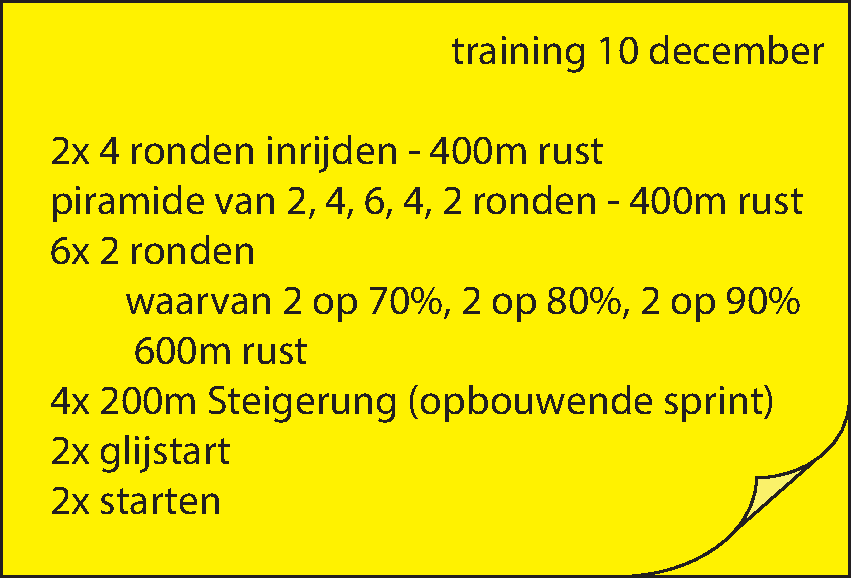
\includegraphics[width=0.4\textwidth]{style/images/training}
  \end{center}
  \caption{Een typisch schaats-trainingsschema}
  \label{fig:training}
\end{figure}

Veel trainingselementen bestaan dus uit korte opdrachten, waar het juist om snelheid gaat. Een enkele lus is dan niet afdoende, omdat de rust voor of na de opdracht mee wordt gewogen. Schaatsers starten en stoppen namelijk niet precies boven de lus, maar starten vaak na de bocht en stoppen afhankelijk van de afstand van de opdracht op een willekeurig punt. 

Andere trainingen van bijvoorbeeld lange afstands- of marathonschaatsers kunnen bestaan uit één element: de hele training lang schaatsen, zonder overeind te komen. Wanneer er op tactische punten detectielussen geïnstalleerd zijn, is het bijvoorbeeld ook mogelijk om onderscheid te maken tussen bochten en de rechte stukken. Bij sporten met een ronde baan verschilt de snelheid in de bocht namelijk erg met die op het rechte eind. Deze vergelijking wordt nu al in Thialf gedaan, maar eigenlijk alleen in het professionele circuit en tijdens wedstrijden op televisie.

Topsporters zijn enorm prestatiegericht en als je al aan de top zit, dan kunnen kleine aanpassingen aan je techniek, ademhaling et cetera, allesbepalende verschillen maken. Coaches van professionele teams houden zich daarom bezig met allerhande analyses. Naast ademanalyse en hartslag monitoring, is het in Thialf bijvoorbeeld ook mogelijk om (van maximaal 20 schaatsers) continu de positie te bepalen met een in-door positioning system (IPS) ontwikkeld door InnoSportLab\footnote{\url{http://www.innosportlabthialf.nl}}.

Al deze geavanceerde analyses zijn echter duur en kosten te veel tijd om aantrekkelijk te zijn voor recreatieve schaatsers. \mylaps X2 kan in combinatie met de applicatie die tijdens dit bachelorproject is gebouwd, recreatieve schaatsers een manier bieden om analyses uit te voeren en hun prestaties naar een hoger niveau te tillen. Het is dan ook de bedoeling dat iedereen met een iPhone vanaf dit schaatsseizoen de Vantage Practice Applicatie kan downloaden vanuit de App Store.

